\documentclass[letterpaper, twoside, 12pt]{book}
\usepackage{packet}


\begin{document}

\setcounter{chapter}{0}

\chapter{Sections 12.1-13.2 INSTRUCTOR SOLUTIONS}

\setcounter{chapter}{12}

\section{Two and Three Dimensional Space}

\begin{definition}
  Let $\mathbb{R}$ be the collection of real numbers, let $\mathbb{R}^2$ be the
  collection of all \textbf{ordered pairs} of real numbers, and let $\mathbb{R}^3$
  be the collection of all \textbf{ordered triples} of real numbers.

  $\mathbb{R}$ is known as the \textbf{real line}, $\mathbb{R}^2$ is known
  as the \textbf{real plane} or the \textbf{$xy$-plane}, and $\mathbb{R}^3$
  is known as \textbf{real (3D) space} or \textbf{$xyz$-space}.
\end{definition}

\begin{center}
  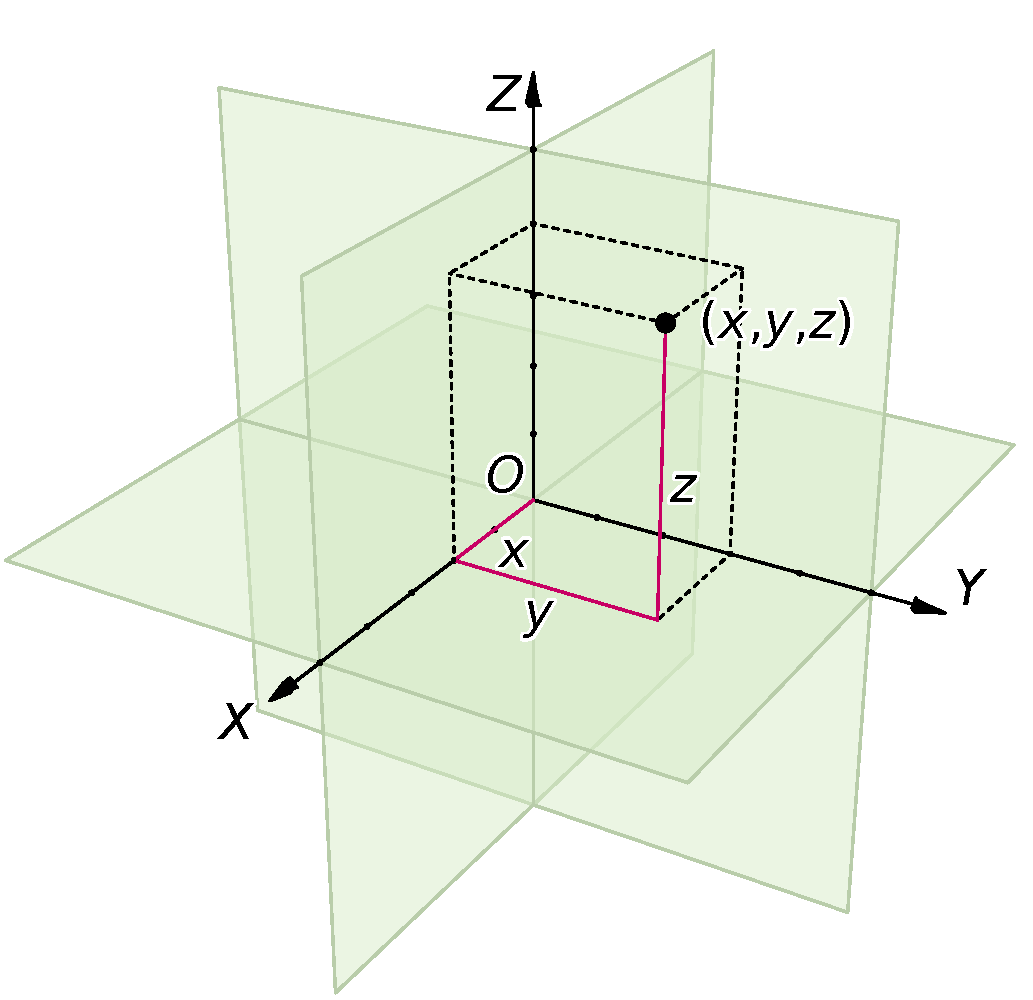
\includegraphics[width=0.5\textwidth]{assets/3dCoordinateSystem.pdf}
\end{center}

\begin{definition}
  The \textbf{distance} between two points $P=(x_1,y_1)$ and
  $Q=(x_2,y_2)$ in $\mathbb{R}^2$ is given by the formula
  \[
    d(P,Q) = \sqrt{(x_2-x_1)^2+(y_2-y_1)^2}
  \]

  The \textbf{distance} between two points $P=(x_1,y_1,z_1)$ and
  $Q=(x_2,y_2,z_2)$ in $\mathbb{R}^3$ is given by the formula
  \[
    d(P,Q) = \sqrt{(x_2-x_1)^2+(y_2-y_1)^2+(z_2-z_1)^2}
  \]
\end{definition}

          \begin{problem}
            Plot and find the distance between the points
            $(-2,6)$ and $(3,-6)$.
          \end{problem}

          \begin{solution}
  The distance between $P=(-2,6)$ and
  $Q=(3,-6)$ is given by the formula
  \[
    d(P,Q) = \sqrt{(3-(-2))^2+(-6-6)^2} = 13
  \]
          \end{solution}

          \begin{problem}
            Plot and find the distance between the points
            $(0,0,0)$ and $(4,2,4)$.
          \end{problem}

          \begin{solution}
  The distance between $P=(0,0,0)$ and
  $Q=(4,2,4)$ is given by the formula
  \[
    d(P,Q) = \sqrt{(4-0)^2+(2-0)^2+(4-0)^2} = 6
  \]
          \end{solution}

          \begin{problem}
            Plot and find the distance between the points
            $(3,7,-2)$ and $(-1,7,1)$.
          \end{problem}

          \begin{solution}
  The distance between $P=(3,7,-2)$ and
  $Q=(-1,7,1)$ is given by the formula
  \[
    d(P,Q) = \sqrt{(-1-3)^2+(7-7)^2+(1-(-2))^2} = 5
  \]
          \end{solution}

          \begin{problem}
            Plot and find the distance between the points
            $(8,2,1)$ and $(4,-2,7)$.
          \end{problem}

          \begin{solution}
  The distance between $P=(8,2,1)$ and
  $Q=(4,-2,7)$ is given by the formula
  \[
    d(P,Q) = \sqrt{(4-8)^2+(-2-2)^2+(7-1)^2} = 2\sqrt{17}
  \]
          \end{solution}





\begin{definition}
  \textbf{Simple lines} in $\mathbb{R}^2$ are given by the relations $x=a$,
  and $y=b$ for real numbers $a,b$.

  \textbf{Simple planes} in $\mathbb{R}^3$ are given by the relations $x=a$,
  $y=b$, $z=c$ for real numbers $a,b,c$.
\end{definition}

\begin{definition}
  A \textbf{circle} in $\mathbb{R}^2$ is the set of all points a fixed distance
  (called its \textbf{radius}) from a fixed point (called its \textbf{center}).
  For a center $(a,b)$ and radius $r$, the equation for a circle is
  \[
    (x-a)^2+(y-b)^2=r^2
  \]

  A \textbf{sphere} in $\mathbb{R}^3$ is the set of all points a fixed distance
  (called its \textbf{radius}) from a fixed point (called its \textbf{center}).
  For a center $(a,b,c)$ and radius $r$, the equation for a sphere is
  \[
    (x-a)^2+(y-b)^2+(z-c)^2=r^2
  \]
\end{definition}

          \begin{problem}
            Plot the curve $x=3$ in the $xy$-plane and the surface
            $x=3$ in $xyz$-space.
          \end{problem}

          \begin{solution}

          \end{solution}

          \begin{problem}
            Plot the curve $y=-1$ in the $xy$-plane and and the surface
            $y=-1$ in $xyz$-space.
          \end{problem}

          \begin{solution}

          \end{solution}

          \begin{problem}
            Plot the surface $z=0$ in $xyz$-space.
          \end{problem}

          \begin{solution}

          \end{solution}

          \begin{problem}
            Plot the curve $(x-2)^2+(y+1)^2=9$ in the $xy$-plane.
          \end{problem}

          \begin{solution}

          \end{solution}

          \begin{problem}
            Plot the surface $x^2+y^2+z^2=4$ in $xyz$-space.
          \end{problem}

          \begin{solution}

          \end{solution}

          \begin{problem}
            Plot the curve $x^2+(y-1)^2+z^2=1$ in $xyz$-space.
          \end{problem}

          \begin{solution}

          \end{solution}



\begin{suggestedHW}
Section $12.1$ numbers $4,$ $6,$ $7,$ $8,$ $10,$ $11,$ $12,$ $14,$ $15,$ $16$
\end{suggestedHW}



\section{Vectors}

\begin{definition}[Vector\index{Vector}]
  A \textbf{vector} $\harpvec v$ is a mathematical object that stores a
  \textbf{magnitude} (a nonnegative real number often thought of as length)
  and \textbf{direction}. Two vectors are \textbf{equal} if and only if they
  have the same magnitude and direction.
\end{definition}

\begin{definition}
  The \textbf{zero vector} $\harpvec0$ has zero magnitude and no direction.
  (This is the only vector without a direction.)
\end{definition}

\begin{definition}
  For a given point $P=(a,b)$ in $\mathbb{R}^2$, its \textbf{position vector}
  is given by $\harpvec{P}=\<a,b\>$: the vector from the origin $(0,0)$ to the
  point $P=(a,b)$.

  For a given point $P=(a,b,c)$ in $\mathbb{R}^3$, its \textbf{position vector}
  is given by $\harpvec{P}=\<a,b,c\>$: the vector from the origin $(0,0,0)$ to
  the point $P=(a,b,c)$.
\end{definition}

\begin{theorem}
  Two vectors are equal if and only if they share the same magnitude and
  direction as a common position vector.
\end{theorem}

\begin{definition}
  Since all vectors are equal to some position vector $\<a,b\>$ or $\<a,b,c\>$,
  we usually define vectors by a position vector written in this
  \textbf{component form}.
  Since the component form of a vector stores the same information as a point,
  we will use both interchangeably, that is, $\<a,b\>=(a,b)\in\mathbb{R}^2$ and
  $\<a,b,c\>=(a,b,c)\in\mathbb{R}^3$
  (although we usually sketch them differently).
\end{definition}

          \begin{problem}
            Plot the point $(1,3)$ and the position vector
            $\<1,3\>$ in the $xy$-plane.
          \end{problem}

          \begin{solution}

          \end{solution}

          \begin{problem}
            Plot the point $(-2,5)$ and the position vector
            $\<-2,5\>$ in the $xy$-plane.
          \end{problem}

          \begin{solution}

          \end{solution}

          \begin{problem}
            Plot the point $(1,1,-3)$ and the position vector
            $\<1,1,-3\>$ in $xyz$-space.
          \end{problem}

          \begin{solution}

          \end{solution}

          \begin{problem}
            Plot the point $(0,5,0)$ and the position vector
            $\<0,5,0\>$ in $xyz$-space.
          \end{problem}

          \begin{solution}

          \end{solution}





\begin{definition}
  Let $P = \left(x_1,y_1,z_1\right)$ and $Q = \left(x_2,y_2,z_2\right).$
  Then the vector with initial point $P$ and terminal point $Q$ is defined as
  \[
    \harpvec{PQ} = \threevec{x_2 - x_1}{y_2 - y_1}{z_2 - z_1}
  \]
\end{definition}

          \begin{problem}
            Plot $P=(1,3)$ and $Q=(-3,6)$ in the $xy$-plane.
            Then compute and plot the vector $\harpvec{PQ}$.
          \end{problem}

          \begin{solution}
  The vector $\vect{PQ}$ is given by
  \[
    \vect{PQ} = \<6-3,-3-1\> = \<3,-4\>
  \]
          \end{solution}

          \begin{problem}
            Plot $P=(3,1)$ and $Q=(0,-2)$ in the $xy$-plane.
            Then compute and plot the vector $\harpvec{PQ}$.
          \end{problem}

          \begin{solution}
  The vector $\vect{PQ}$ is given by
  \[
    \vect{PQ} = \<0-3,-2-1\> = \<-3,-3\>
  \]
          \end{solution}

          \begin{problem}
            Plot $P=(1,1,1)$ and $Q=(-3,-1,3)$ in $xyz$-space.
            Then compute and plot the vector $\harpvec{PQ}$.
          \end{problem}

          \begin{solution}
  The vector $\vect{PQ}$ is given by
  \[
    \vect{PQ} = \<-3-1,-1-1,3-1\> = \<-4,-2,2\>
  \]
          \end{solution}

          \begin{problem}
            Plot $P=(-2,0,3)$ and $Q=(1,3,-3)$ in $xyz$-space.
            Then compute and plot the vector $\harpvec{PQ}$.
          \end{problem}

          \begin{solution}
  The vector $\vect{PQ}$ is given by
  \[
    \vect{PQ} = \<1-(-2),3-0,-3-3\> = \<-3,3,-6\>
  \]
          \end{solution}



\begin{definition}
  The magnitude $|\harpvec{v}|$ of a vector $\harpvec{v}$ in $\mathbb{R}^2$ or
  $\mathbb{R}^3$ is the distance between its initial and terminal points.
\end{definition}

\begin{theorem}
  The magnitude of $\harpvec{v}=\<a,b\>$ is given by
    \[|\harpvec{v}|=\sqrt{a^2+b^2}\]

  The magnitude of $\harpvec{v}=\<a,b,c\>$ is given by
    \[|\harpvec{v}|=\sqrt{a^2+b^2+c^2}\]
\end{theorem}



          \begin{problem}
            Evaluate the magnitude of the position vector $\<5,5\>$.
          \end{problem}

          \begin{solution}
  The magnitude of $\vect{v}=\<5,5\>$ is given by
  \[|\vect{v}|=\sqrt{5^2+5^2}=5\sqrt{2}\]
          \end{solution}

          \begin{problem}
            Evaluate the magnitude of the position vector $\<-4,3\>$.
          \end{problem}

          \begin{solution}
  The magnitude of $\vect{v}=\<-4,3\>$ is given by
  \[|\vect{v}|=\sqrt{(-4)^2+3^2}=5\]
          \end{solution}

          \begin{problem}
            Evaluate the magnitude of the position vector $\<12,-5\>$.
          \end{problem}

          \begin{solution}
  The magnitude of $\vect{v}=\<12,-5\>$ is given by
  \[|\vect{v}|=\sqrt{12^2+(-5)^2}=13\]
          \end{solution}

          \begin{problem}
            Evaluate the magnitude of the position vector $\<3,1,-2\>$.
          \end{problem}

          \begin{solution}
  The magnitude of $\vect{v}=\<3,1,-2\>$ is given by
  \[|\vect{v}|=\sqrt{3^2+1^2+(-2)^2}=\sqrt{14}\]
          \end{solution}

          \begin{problem}
            Evaluate the magnitude of the position vector $\<4,-2,-4\>$.
          \end{problem}

          \begin{solution}
  The magnitude of $\vect{v}=\<4,-2,-4\>$ is given by
  \[|\vect{v}|=\sqrt{4^2+(-2)^2+(-4)^2}=6\]
          \end{solution}

          \begin{problem}
            Evaluate the magnitude of the position vector $\<8,0,-6\>$.
          \end{problem}

          \begin{solution}
  The magnitude of $\vect{v}=\<8,0,-6\>$ is given by
  \[|\vect{v}|=\sqrt{8^2+0^2+(-6)^2}=10\]
          \end{solution}



\begin{definition}
  \textbf{Vector addition} is defined component-wise as follows for
  $\mathbb{R}^2$ and $\mathbb{R}^3$
  \[
    \harpvec{u}+\harpvec{v}
      =
    \<u_1,u_2\>+\<v_1,v_2\>
      =
    \<u_1+v_1,u_2+v_2\>
  \]
  \[
    \harpvec{u}+\harpvec{v}
      =
    \<u_1,u_2,u_3\>+\<v_1,v_2,v_3\>
      =
    \<u_1+v_1,u_2+v_2,u_3+v_3\>
  \]
\end{definition}

\begin{definition}
  A \textbf{scalar} is simply a real number by itself
  (as opposed to a vector of real numbers).
\end{definition}

\begin{definition}
  \textbf{Scalar multiplication of a vector} is defined component-wise as
  follows for $\mathbb{R}^2$ and $\mathbb{R}^3$:
  \[
    k\harpvec{u}
      =
    k\<u_1,u_2\>
      =
    \<ku_1,ku_2\>
  \]
  \[
    k\harpvec{u}
      =
    k\<u_1,u_2,u_3\>
      =
    \<ku_1,ku_2,ku_3\>
  \]
\end{definition}



          \begin{problem}
            Compute and plot $\harpvec{u}=\<1,-3\>$, $\harpvec{v}=\<3,1\>$
            and $\harpvec{u}+\harpvec{v}$ in the $xy$-plane.
          \end{problem}

          \begin{solution}
  The vector $\harpvec{u}+\harpvec{v}$ is given by
  \[
    \<1,-3\>+\<3,1\>=\<1+3,-3+1\>=\<4,-2\>
  \]
          \end{solution}

          \begin{problem}
            Compute and plot $\harpvec{u}=\<2,0,1\>$, $\harpvec{v}=\<-2,4,2\>$
            and $\harpvec{u}+\harpvec{v}$ in $xyz$-space.
          \end{problem}

          \begin{solution}
  The vector $\harpvec{u}+\harpvec{v}$ is given by
  \[
    \<2,0,1\>+\<-2,4,2\>=\<2-2,0+4,1+2\>=\<0,4,3\>
  \]
          \end{solution}

          \begin{problem}
            Compute and plot $\harpvec{u}=\<8,-2\>$ and
            $\frac{1}{2}\harpvec{u}$ in the $xy$-plane.
          \end{problem}

          \begin{solution}
  The vector $\frac{1}{2}\harpvec{u}$ is given by
  \[
    \frac{1}{2}\<8,-2\>=\left\<\frac{1}{2}8,\frac{1}{2}(-2)\right\>=\<4,-1\>
  \]
          \end{solution}

          \begin{problem}
            Compute and plot $\harpvec{u}=\<5,3,-1\>$ and
            $3\harpvec{u}$ in $xyz$-space.
          \end{problem}

          \begin{solution}
  The vector $3\harpvec{u}$ is given by
  \[
    3\<5,3,-1\>=\<3(5),3(3),3(-1)\>=\<15,9,-3\>
  \]
          \end{solution}



\begin{definition}
  A vector $\harpvec{v}$ is a \textbf{unit vector} if $|\harpvec v|=1$.
\end{definition}

\begin{theorem}
  For any non-zero vector $\harpvec{v}$, the vector
  \[
    \frac{1}{|\harpvec v|}\harpvec{v} = \frac{\harpvec v}{|\harpvec v|}
  \]
  is a unit vector.
\end{theorem}

\begin{definition}
  The \textbf{direction} of a vector $\harpvec v$ is the unit vector
  $\frac{\harpvec v}{|\harpvec v|}$.
\end{definition}

\begin{theorem}
  Any vector $\harpvec v$ is the scalar product of its magnitude and direction:
  \[
    \harpvec v = |\harpvec v|\frac{\harpvec v}{|\harpvec v|}
  \]
\end{theorem}



          \begin{problem}
            Rewrite $\<5,5\>$ as the scalar product of its magnitude and
            direction.
          \end{problem}

          \begin{solution}
  The magnitude of $\vect{v}=\<5,5\>$ is given by
  \[|\vect{v}|=\sqrt{5^2+5^2}=5\sqrt{2}\]

  The direction of $\vect{v}=\<5,5\>$ is then given by
  \[
  \frac{\harpvec v}{|\harpvec v|}
    =
  \frac{\<5,5\>}{5\sqrt{2}}
    =
  \left\<\frac{5}{5\sqrt{2}},\frac{5}{5\sqrt{2}}\right\>
    =
  \left\<\frac{1}{\sqrt{2}},\frac{1}{\sqrt{2}}\right\>
  \]

  Therefore
  \[
    \<5,5\>
      =
    5\sqrt{2}\left\<\frac{1}{\sqrt{2}},\frac{1}{\sqrt{2}}\right\>
  \]
          \end{solution}

          \begin{problem}
            Rewrite $\<-4,3\>$ as the scalar product of its magnitude and
            direction.
          \end{problem}

          \begin{solution}
  The magnitude of $\vect{v}=\<-4,3\>$ is given by
  \[|\vect{v}|=\sqrt{(-4)^2+3^2}=5\]

  The direction of $\vect{v}=\<-4,3\>$ is then given by
  \[
  \frac{\harpvec v}{|\harpvec v|}
    =
  \frac{\<-4,3\>}{5}
    =
  \left\<-\frac{4}{5},\frac{3}{5}\right\>
  \]

  Therefore
  \[
    \<-4,3\>
      =
    5\left\<-\frac{4}{5},\frac{3}{5}\right\>
  \]
          \end{solution}

          \begin{problem}
            Rewrite $\<12,-5\>$ as the scalar product of its magnitude and
            direction.
          \end{problem}

          \begin{solution}
  The magnitude of $\vect{v}=\<12,-5\>$ is given by
  \[|\vect{v}|=\sqrt{12^2+(-5)^2}=13\]

  The direction of $\vect{v}=\<12,-5\>$ is then given by
  \[
  \frac{\harpvec v}{|\harpvec v|}
    =
  \frac{\<12,-5\>}{13}
    =
  \left\<\frac{12}{13},-\frac{5}{13}\right\>
  \]

  Therefore
  \[
    \<12,-5\>
      =
    13\left\<\frac{12}{13},-\frac{5}{13}\right\>
  \]
          \end{solution}

          \begin{problem}
            Rewrite $\<3,1,-2\>$ as the scalar product of its magnitude and
            direction.
          \end{problem}

          \begin{solution}
  The magnitude of $\vect{v}=\<3,1,-2\>$ is given by
  \[|\vect{v}|=\sqrt{3^2+1^2+(-2)^2}=\sqrt{14}\]

  The direction of $\vect{v}=\<12,-5\>$ is then given by
  \[
  \frac{\harpvec v}{|\harpvec v|}
    =
  \frac{\<3,1,-2\>}{\sqrt{14}}
    =
  \left\<\frac{3}{\sqrt{14}},\frac{1}{\sqrt{14}},-\frac{2}{\sqrt{14}}\right\>
  \]

  Therefore
  \[
    \<3,1,-2\>
      =
    \sqrt{14}
    \left\<\frac{3}{\sqrt{14}},\frac{1}{\sqrt{14}},-\frac{2}{\sqrt{14}}\right\>
  \]
          \end{solution}

          \begin{problem}
            Rewrite $\<4,-2,-4\>$ as the scalar product of its magnitude and
            direction.
          \end{problem}

          \begin{solution}
  The magnitude of $\vect{v}=\<4,-2,-4\>$ is given by
  \[|\vect{v}|=\sqrt{4^2+(-2)^2+(-4)^2}=6\]

  The direction of $\vect{v}=\<4,-2,-4\>$ is then given by
  \[
  \frac{\harpvec v}{|\harpvec v|}
    =
  \frac{\<4,-2,-4\>}{6}
    =
  \left\<\frac{4}{6},-\frac{2}{6},-\frac{4}{6}\right\>
    =
  \left\<\frac{2}{3},-\frac{1}{3},-\frac{2}{3}\right\>
  \]

  Therefore
  \[
    \<4,-2,-4\>
      =
    6
    \left\<\frac{2}{3},-\frac{1}{3},-\frac{2}{3}\right\>
  \]
          \end{solution}

          \begin{problem}
            Rewrite $\<8,0,-6\>$ as the scalar product of its magnitude and
            direction.
          \end{problem}

          \begin{solution}
  The magnitude of $\vect{v}=\<8,0,-6\>$ is given by
  \[|\vect{v}|=\sqrt{8^2+0^2+(-6)^2}=10\]

  The direction of $\vect{v}=\<8,0,-6\>$ is then given by
  \[
  \frac{\harpvec v}{|\harpvec v|}
    =
  \frac{\<8,0,-6\>}{10}
    =
  \left\<\frac{8}{10},\frac{0}{10},-\frac{6}{10}\right\>
    =
  \left\<\frac{4}{5},0,-\frac{3}{5}\right\>
  \]

  Therefore
  \[
    \<8,0,-6\>
      =
    10
    \left\<\frac{4}{5},0,-\frac{3}{5}\right\>
  \]
          \end{solution}



\begin{definition}
The \textbf{standard unit vectors} in $\mathbb{R}^2$ are
$\veci=\<1,0\>$ and $\vecj=\<0,1\>$, and any vector in $\mathbb{R}^2$
can be expressed in \textbf{standard unit vector form}:
  \[\<a,b\>=a\veci+b\vecj\]

The \textbf{standard unit vectors} in $\mathbb{R}^3$ are
$\veci=\<1,0,0\>$, $\vecj=\<0,1,0\>$, and $\veck=\<0,0,1\>$, and any vector in
$\mathbb{R}^3$ can be expressed in \textbf{standard unit vector form}:
  \[\<a,b,c\>=a\veci+b\vecj+c\veck\]
\end{definition}

\begin{remark}
  Since the $xy$-plane is the the plane $z=0$ in $xyz$-space, we say the
  points and vectors $(a,b)=(a,b,0)=\<a,b\>=\<a,b,0\>=a\veci+b\vecj+0\veck$
  are all equal.
\end{remark}



          \begin{problem}
            Rewrite $\<5,5\>$ in standard unit vector form.
          \end{problem}

          \begin{solution}
  As $\<a,b\>=a\veci+b\vecj$:
  \[
    \<5,5\>=5\veci+5\vecj
  \]
          \end{solution}

          \begin{problem}
            Rewrite $\<-4,3\>$ in standard unit vector form.
          \end{problem}

          \begin{solution}
  As $\<a,b\>=a\veci+b\vecj$:
  \[
    \<-4,3\>=-4\veci+3\vecj
  \]
          \end{solution}

          \begin{problem}
            Rewrite $\<3,1,-2\>$ in standard unit vector form.
          \end{problem}

          \begin{solution}
  As $\<a,b,c\>=a\veci+b\vecj+c\veck$:
  \[
    \<3,1,-2\>=3\veci+\vecj-2\veck
  \]
          \end{solution}

          \begin{problem}
            Rewrite $\<8,0,-6\>$ in standard unit vector form.
          \end{problem}

          \begin{solution}
  As $\<a,b,c\>=a\veci+b\vecj+c\veck$:
  \[
    \<8,0,-6\>=8\veci+0\vecj-6\veck=8\veci-6\veck
  \]
          \end{solution}



\begin{theorem}
The following properties hold for any two vectors $\harpvec{u}$, $\harpvec{v}$
and scalars $a$, $b$.
  \begin{itemize}
  \item $\harpvec{u}+\harpvec{v} = \harpvec{v}+\harpvec{u}$
  \item $(\harpvec{u}+\harpvec{v})+\harpvec{w} = \harpvec{u}+(\harpvec{v}+\harpvec{w})$
  \item $\harpvec{u}+\harpvec{0} = \harpvec{u}$
  \item $\harpvec{u}+(-\harpvec{u}) = \harpvec{0}$
  \item $0\harpvec{u} = \harpvec{0}$
  \item $1\harpvec{u} = \harpvec{u}$
  \item $a(b\harpvec{u}) = (ab)\harpvec{u}$
  \item $a(\harpvec{u} + \harpvec{v}) = a\harpvec{u} + a\harpvec{v}$
  \item $(a+b)\harpvec{u} = a\harpvec{u} + b\harpvec{u}$
  \end{itemize}
\end{theorem}

\begin{definition}
  \textbf{Vector subtraction} is defined as the addition of a negative:
  \[
    \harpvec{u}-\harpvec{v}
      =
    \harpvec{u}+(-\harpvec{v})
      =
    \<u_1-v_1,u_2-v_2\>
  \]
  \[
    \harpvec{u}-\harpvec{v}
      =
    \harpvec{u}+(-\harpvec{v})
      =
    \<u_1-v_1,u_2-v_2,u_3-v_3\>
  \]
\end{definition}

\begin{suggestedHW}
Section $12.2$ numbers $3,$ $5,$ $13,$ $14,$ $15,$ $19,$ $21,$ $24,$ $26$
\end{suggestedHW}



\section{The Dot Product}

\begin{definition}
  Let $\theta$ be the angle between two non-zero vectors $\harpvec{u}$, $\harpvec{v}$.
  The \textbf{dot product} $\harpvec{u}\cdot\harpvec{v}$ is the product of their
  lengths when projected into the same direction, obtained by this formula:
  \[
    \harpvec{u} \cdot \harpvec{v} = |\harpvec{u}||\harpvec{v}|\cos \theta
  \]
\end{definition}

\begin{definition}
  The dot product with a zero vector is always zero:
  \[\harpvec{v}\cdot\harpvec{0}=\harpvec{0}\cdot\harpvec{v}=0\]
\end{definition}

\begin{theorem}
By the Law of Cosines:
  \[
    \harpvec{u} \cdot \harpvec{v}
      =
    \<u_1,u_2\>\cdot\<v_1,v_2\>
      =
    u_1v_1 + u_2v_2
  \]
  \[
    \harpvec{u} \cdot \harpvec{v}
      =
    \<u_1,u_2,u_3\>\cdot\<v_1,v_2,v_3\>
      =
    u_1v_1 + u_2v_2 + u_3v_3
  \]
\end{theorem}

\begin{definition}
  Two vectors $\harpvec{u},\harpvec{v}$ are \textbf{orthogonal} if
  $\harpvec{u} \cdot \harpvec{v} = 0$.
\end{definition}

\begin{theorem}
  Two non-zero vectors are orthogonal if the angle $\theta$ between them
  is $\frac{\pi}{2}$ radians.
\end{theorem}

\begin{theorem}
The following properties hold for any three vectors $\harpvec{u}$, $\harpvec{v}$,
$\harpvec{w}$ and scalar $c$.
  \begin{itemize}
  \item $\harpvec{u} \cdot \harpvec{v} = \harpvec{v}\cdot\harpvec{u}$
  \item $(c\harpvec{u})\cdot \harpvec{v} = \harpvec{u} \cdot (c\harpvec{v}) = c(\harpvec{u} \cdot \harpvec{v})$
  \item $\harpvec{u} \cdot (\harpvec{v} + \harpvec{w}) = \harpvec{u}\cdot\harpvec{v} + \harpvec{u}\cdot \harpvec{w}$
  \item $\harpvec{u} \cdot \harpvec{u} = |\harpvec{u}|^2$
  \end{itemize}
\end{theorem}

          \begin{problem}
            Compute the angle between the vectors
            $\harpvec{u}=\<4,-3\>$ and $\harpvec{v}=\<5,12\>$.
          \end{problem}

          \begin{solution}
            Note that $|\vect{u}|=|\<4,-3\>|=5$ and
            $|\vect{v}|=|\<5,12\>|=13$.

            By the definition of the dot product:
            \[
              \vect{u}\cdot\vect{v}
                =
              |\vect u||\vect v|\cos\theta
                =
              5(13)\cos\theta
                =
              65\cos\theta
            \]

            By Theorem 64:
            \[
              \vect{u}\cdot\vect{v}
                =
              4(5)+(-3)(12)
                =
              -16
            \]

            We set these equal and solve for $\theta$ as follows:
            \[
              65\cos\theta = -16
            \]
            \[
              \cos\theta = -\frac{16}{65}
            \]
            \[
              \theta = \arccos\left(-\frac{16}{65}\right)
              \approx 1.82 \text{ (radians)}
              \approx 104.3^\circ
            \]
          \end{solution}

          \begin{problem}
            Compute the angle between the vectors
            $\harpvec{u}=\<1,4,2\>$ and $\harpvec{v}=\<4,1,-2\>$.
          \end{problem}

          \begin{solution}
            Note that $|\vect{u}|=|\<1,4,2\>|=\sqrt{21}$ and
            $|\vect{v}|=|\<4,1,-2\>|=\sqrt{21}$.

            By the definition of the dot product:
            \[
              \vect{u}\cdot\vect{v}
                =
              |\vect u||\vect v|\cos\theta
                =
              \sqrt{21}\sqrt{21}\cos\theta
                =
              21\cos\theta
            \]

            By Theorem 64:
            \[
              \vect{u}\cdot\vect{v}
                =
              1(4)+4(1)+(2)(-2)
                =
              4
            \]

            We set these equal and solve for $\theta$ as follows:
            \[
              21\cos\theta = 4
            \]
            \[
              \cos\theta = \frac{4}{21}
            \]
            \[
              \theta = \arccos\left(\frac{4}{21}\right)
              \approx 1.38 \text{ (radians)}
              \approx 79.02^\circ
            \]
          \end{solution}

          \begin{problem}
            Compute the angle between the vectors
            $\harpvec{u}=\<0,5,-11\>$ and $\harpvec{v}=\<2,0,0\>$.
          \end{problem}

          \begin{solution}
            By Theorem 64:
            \[
              \vect{u}\cdot\vect{v}
                =
              0(2)+5(0)+(-11)(0)
                =
              0
            \]

            Therefore $\vect{u},\vect{v}$ are orthogonal,
            and thus $\theta=\frac{\pi}{2}=90^\circ$ by Theorem 66.

            (Note: could also solve the same way as previous problems.)
          \end{solution}



\begin{definition}
The work $W$ done by a force vector $\harpvec{F}$ over a displacement
vector $\harpvec{D}$ is given by
\[
  W = \harpvec{F} \cdot \harpvec{D}
    =
  |\harpvec{F}||\harpvec{D}|\cos \theta
\]
\end{definition}

\begin{suggestedHW}
Section $12.3$ numbers
$3,$ $5,$ $6,$ $7,$ $8,$ $9,$ $10,$ $11,$ $15,$ $17,$
$21,$ $27,$ $41,$ $42,$ $44$
\end{suggestedHW}





\section{The Cross Product}

\begin{definition}
  For any two non-parallel vectors $\harpvec{u}$, $\harpvec{v}$ in $\mathbb R^3$,
  the \textbf{Right-Hand Rule} gives a specific direction orthogonal to both:
  position $\harpvec{u}$ with your right thumb and $\harpvec{v}$ with your
  right index finger, and let your middle finger extend orthogonal to both
  to give this direction.
\end{definition}

\begin{definition}
  Let $\theta$ be the angle between two non-zero vectors $\harpvec{u}$,
  $\harpvec{v}$ in $\mathbb{R}^3$, and let $\harpvec{n}$ be the direction
  given by the Right-Hand Rule.
  The \textbf{cross product} $\harpvec{u}\times\harpvec{v}$ is the vector
  orthogonal to both which follows the Right-Hand Rule and has magnitude
  equal to the area of the parallelogram formed from both.
  \[
    \harpvec{u}\times\harpvec{v}
      =
    (|\harpvec{u}||\harpvec{v}|\sin\theta)\harpvec{n}
  \]
  \[
    |\harpvec{u}\times\harpvec{v}|
      =
    |\harpvec{u}||\harpvec{v}|\sin\theta
  \]
\end{definition}

\begin{definition}
  The cross product with a zero vector is always the zero vector:
  \[\harpvec{v}\times\harpvec{0}=\harpvec{0}\times\harpvec{v}=\harpvec{0}\]
\end{definition}

\begin{theorem}
  The following properties hold for any three vectors $\harpvec{u}$, $\harpvec{v}$,
  $\harpvec{w}$ and scalars $a$,$b$.
  \begin{itemize}
  \item $(a\harpvec{u}) \times (b\harpvec{v}) = (ab)(\harpvec{u} \times \harpvec{v})$
  \item
    $\harpvec{u} \times (\harpvec{v} + \harpvec{w}) =
    \harpvec{u} \times \harpvec{v} + \harpvec{u} \times \harpvec{w}$
  \item
    $(\harpvec{v} + \harpvec{w}) \times \harpvec{u} =
    \harpvec{v} \times \harpvec{u} + \harpvec{w} \times \harpvec{u}$
  \item $\harpvec{v} \times \harpvec{u} = -(\harpvec{u} \times \harpvec{v})$
  \end{itemize}
\end{theorem}

\begin{definition}
  Two vectors $\harpvec{u},\harpvec{v}$ are \textbf{parallel} if
  $\harpvec{u} \times \harpvec{v} = 0$.
\end{definition}

\begin{theorem}
  Two non-zero vectors are parallel if the angle $\theta$ between them
  is $0$ or $\pi$ radians.
\end{theorem}

\begin{definition}
  The cross products of the standard unit vectors are given as follows:
  \begin{itemize}
    \item $\veci \times \vecj = \veck$
    \item $\vecj \times \veck = \veci$
    \item $\veck \times \veci = \vecj$
  \end{itemize}
\end{definition}

\begin{definition}
  A \textbf{determinant} is a short hand for writing certain commonly
  occuring algebraic expressions:
    \[
      \begin{array}{|c c|}
      a_1 & a_2 \\
      b_1 & b_2 \\
      \end{array}
        =
      a_1b_2 - a_2b_1
    \]
    \[
      \begin{array}{|c c c|}
      a_1 & a_2 & a_3 \\
      b_1 & b_2 & b_3 \\
      c_1 & c_2 & c_3 \\
      \end{array}
        =
      a_1 \,
      \begin{array}{|c c|}
      b_2 & b_3 \\
      c_2 & c_3 \\
      \end{array}
        -
      a_2 \,
      \begin{array}{|c c|}
      b_1 & b_3 \\
      c_1 & c_3 \\
      \end{array}
        +
      a_3 \,
      \begin{array}{|c c|}
      b_1 & b_2 \\
      c_1 & c_2 \\
      \end{array}
    \]
\end{definition}



\begin{theorem}
  By breaking up $\harpvec{u}$, $\harpvec{v}$ into standard unit vectors:
  \[
  \harpvec{u} \times \harpvec{v}
    =
  \begin{array}{|c c c|}
  \veci & \vecj & \veck \\
  u_1 & u_2 & u_3 \\
  v_1 & v_2 & v_3 \\
  \end{array}
    =
  \left\<
    \begin{array}{|c c|}
    u_2 & u_3 \\
    v_2 & v_3 \\
    \end{array}
      \,,-\,
    \begin{array}{|c c|}
    u_1 & u_3 \\
    v_1 & v_3 \\
    \end{array}
      \,,\,
    \begin{array}{|c c|}
    u_1 & u_2 \\
    v_1 & v_2 \\
    \end{array}
  \right\>
  \]
\end{theorem}

          \begin{problem}
            Compute a nonzero vector normal to both $\harpvec{u}=\<4,-3,0\>$
            and $\harpvec{v}=\<2,6,-3\>$.
          \end{problem}

          \begin{solution}
  The cross-product is always normal to its factors. Therefore

  \[
  \vect{u}\times\vect{v}
    =
  \begin{array}{|c c c|}
  \veci & \vecj & \veck \\
  4   & -3  & 0   \\
  2   & 6   & -3  \\
  \end{array}
    =
  \left\<
    \begin{array}{|c c|}
    -3  & 0   \\
    6   & -3  \\
    \end{array}
      \,,-\,
    \begin{array}{|c c|}
    4   & 0   \\
    2   & -3  \\
    \end{array}
      \,,\,
    \begin{array}{|c c|}
    4   & -3  \\
    2   & 6   \\
    \end{array}
  \right\>
  \]
  \[
    =
  \<9-0,-(-12-0),24-(-6)\>
    =
  \<9,12,30\>
  \]
  is normal to both $\vect{u},\vect{v}$.
          \end{solution}

          \begin{problem}
            Compute a nonzero vector normal to both $\harpvec{u}=\<1,4,2\>$
            and $\harpvec{v}=\<4,1,-2\>$.
          \end{problem}

          \begin{solution}
  The cross-product is always normal to its factors. Therefore

  \[
  \vect{u}\times\vect{v}
    =
  \begin{array}{|c c c|}
  \veci & \vecj & \veck \\
  1   & 4   & 2   \\
  4   & 1   & -2  \\
  \end{array}
    =
  \left\<
    \begin{array}{|c c|}
    4   & 2   \\
    1   & -2  \\
    \end{array}
      \,,-\,
    \begin{array}{|c c|}
    1   & 2   \\
    4   & -2  \\
    \end{array}
      \,,\,
    \begin{array}{|c c|}
    1   & 4   \\
    4   & 1   \\
    \end{array}
  \right\>
  \]
  \[
    =
  \<-8-2,-(-2-8),1-16\>
    =
  \<-10,10,-15\>
  \]
  is normal to both $\vect{u},\vect{v}$.
          \end{solution}

          \begin{problem}
            Compute a nonzero vector normal to both $\harpvec{u}=\<0,5,-11\>$
            and $\harpvec{v}=\<2,0,0\>$.
          \end{problem}

          \begin{solution}
  The cross-product is always normal to its factors. Therefore

  \[
  \vect{u}\times\vect{v}
    =
  \begin{array}{|c c c|}
  \veci & \vecj & \veck \\
  0   & 5   & -11 \\
  2   & 0   & 0   \\
  \end{array}
    =
  \left\<
    \begin{array}{|c c|}
    5   & -11 \\
    0   & 0   \\
    \end{array}
      \,,-\,
    \begin{array}{|c c|}
    0   & -11 \\
    2   & 0   \\
    \end{array}
      \,,\,
    \begin{array}{|c c|}
    0   & 5   \\
    2   & 0   \\
    \end{array}
  \right\>
  \]
  \[
    =
  \<0-0,-(0-(-22)),0-10\>
    =
  \<0,-22,-10\>
  \]
  is normal to both $\vect{u},\vect{v}$.
          \end{solution}



\begin{definition}
  The torque $\tau$ done by a force vector $\harpvec{F}$ on an arm given by
  $\harpvec{D}$ is given by
  \[
    \tau = |\harpvec{F} \times \harpvec{D}|
      =
    |\harpvec{F}||\harpvec{D}|\sin \theta
  \]
\end{definition}

\begin{theorem}
  The volume of a parallelpiped determined by the vectors
  $\harpvec{u}$, $\harpvec{v}$, $\harpvec{w}$, is given by
  the \textbf{triple scalar product}
    \[
      (\harpvec{u}\times\harpvec{v})\cdot\harpvec{w} =
      \begin{array}{|c c c|}
      u_1 & u_2 & u_3 \\
      v_1 & v_2 & v_3 \\
      w_1 & w_2 & w_3 \\
      \end{array}
    \]
\end{theorem}

\begin{suggestedHW}
  Section $12.4$ numbers $1 - 3,$ $17,$ $19,$ $28,$ $29,$ $33,$ $35$
\end{suggestedHW}



\section{Lines and Planes in Space}

\begin{theorem}
  Let $L$ be the line in $\mathbb R^2$ normal to the vector $\harpvec N=\<A,B\>$
  and passing through the point $P_0=(x_0,y_0)$. Then every point $P=(x,y)$
  on the line $L$ must satisfy the following equations:
  \[
    \harpvec N \cdot \harpvec{P_0P} = 0
  \]
  \[
    A(x-x_0) + B(y-y_0) = 0
  \]

  Let $M$ be the plane in $\mathbb R^3$ normal to the vector $\harpvec N=\<A,B,C\>$
  and passing through the point $P_0=(x_0,y_0,z_0)$. Then every point $P=(x,y,z)$
  on the plane $M$ must satisfy the following equations:
  \[
    \harpvec N \cdot \harpvec{P_0P} = 0
  \]
  \[
    A(x-x_0) + B(y-y_0) + C(z-z_0) = 0
  \]
\end{theorem}

          \begin{problem}
            Find an equation for the line passing through $(1,-2)$ and parallel
            to the line with equation $2x-y=3$. Then plot both lines.
          \end{problem}

          \begin{solution}
  The line with equation $2x-y=3$ has a normal vector $\<2,-1\>$,
  so any line parallel to it would have the same normal vector.

  Using the point $(1,-2)$ and the normal vector $\<2,-1\>$,
  this line has the equation (by Theorem 86):
  \[
    2(x-1) + -1(y-(-2)) = 0
  \]
  \[
    2x - y = 4
  \]
          \end{solution}

          \begin{problem}
            Find an equation for the plane passing through $(1,3,-2)$ and
            normal to the vector $\<3,0,1\>$. Then plot the plane and vector.
          \end{problem}

          \begin{solution}
  Using the point $(1,3,-2)$ and the normal vector $\<3,0,1\>$,
  such a plane has the equation (by Theorem 86):
  \[
    3(x-1) + 0(y-3) + 1(z-(-2)) = 0
  \]
  \[
    3x + z = 1
  \]
          \end{solution}

          \begin{problem}
            Find an equation for the plane passing through $(-2,0,4)$,
            $(1,3,3)$, and $(0,0,2)$. Then plot the plane and points.
          \end{problem}

          \begin{solution}
  Let $P=(-2,0,4)$, $Q=(1,3,3)$, and $R=(0,0,2)$ denote the given points
  on the plane. Then
  $\vect{PQ}\times\vect{PR}=\<3,3,-1\>\times\<2,0,-2\>$
  is normal to the plane.

  \[
  \vect{PQ}\times\vect{PR}
    =
  \begin{array}{|c c c|}
  \veci & \vecj & \veck \\
  3   & 3   & -1  \\
  2   & 0   & -2  \\
  \end{array}
    =
  \left\<
    \begin{array}{|c c|}
    3   & -1  \\
    0   & -2  \\
    \end{array}
      \,,-\,
    \begin{array}{|c c|}
    3   & -1  \\
    2   & -2  \\
    \end{array}
      \,,\,
    \begin{array}{|c c|}
    3   & 3   \\
    2   & 0   \\
    \end{array}
  \right\>
  \]
  \[
    =
  \<-6-0,-(-6-(-2)),0-6\>
    =
  \<-6,4,-6\>
  \]

  Using the point $(0,0,2)$ (any other point would also work)
  and the normal vector $\<-6,4,-6\>$,
  such a plane has the equation (by Theorem 86):
  \[
    -6(x-0) + 4(y-0) + -6(z-2) = 0
  \]
  \[
    -6x + 4y - 6z = -12
  \]
  \[
    -3x + 2y - 3z = -6
  \]
          \end{solution}



\begin{definition}
  \textbf{Parametric equations} $x(t),y(t)$
  for a curve in $\mathbb R^2$ assign a point $(x(t),y(t))$ of the curve
  to each value of $t$.

  \textbf{Parametric equations} $x(t),y(t),z(t)$
  for a curve in $\mathbb R^3$ assign a point $(x(t),y(t),z(t))$ of the curve
  to each value of $t$.
\end{definition}



          \begin{problem}
            Sketch the curve given by the parametric equations
            $x(t)=t$ and $y(t)=t^2$.
          \end{problem}

          \begin{solution}

          \end{solution}

          \begin{problem}
            Sketch the curve given by the parametric equations
            $x(t)=\sin t$ and $y(t)=\frac{t}{\pi}$.
          \end{problem}

          \begin{solution}

          \end{solution}

          \begin{problem}
            Sketch the curve given by the parametric equations
            $x(t)=1-t$, $y(t)=3t$, and $z(t)=2t-3$.
          \end{problem}

          \begin{solution}

          \end{solution}

          \begin{problem}
            Sketch the curve given by the parametric equations
            $x(t)=-t^2$, $y(t)=2$, and $z(t)=t$.
          \end{problem}

          \begin{solution}

          \end{solution}



\begin{theorem}
  Let $L$ be the line in $\mathbb R^2$ parallel to the vector $\harpvec v=\<a,b\>$
  and passing through the point $P_0=(x_0,y_0)$. Then every point $P=(x,y)$
  on the line $L$ must satisfy the following vector equation for some $t$:
  \[
    \harpvec{P} = \harpvec{v}t + \harpvec{P_0}
  \]
  Thus the line is given by the parametric equations
  \[
    x(t) = at + x_0
  \]
  \[
    y(t) = bt + y_0
  \]

  Let $L$ be the line in $\mathbb R^3$ parallel to the vector $\harpvec v=\<a,b,c\>$
  and passing through the point $P_0=(x_0,y_0,z_0)$. Then every point $P=(x,y,z)$
  on the line $L$ must satisfy the following vector equation for some $t$:
  \[
    \harpvec{P} = \harpvec{v}t + \harpvec{P_0}
  \]
  Thus the line is given by the parametric equations
  \[
    x(t) = at + x_0
  \]
  \[
    y(t) = bt + y_0
  \]
  \[
    z(t) = ct + z_0
  \]
\end{theorem}



          \begin{problem}
            Find parametric equations for the line with equation $y=-3x+1$
            in the $xy$ plane. Then plot the line.
          \end{problem}

          \begin{solution}
  The $y$-intercept for this line is the point $(0,1)$.

  The slope of this line is $-3$, so it has a rise of $-3$ for a run of $1$.
  Therefore $\<1,-3\>$ is a parallel vector to this line.

  Parametric equations for a line passing through $(0,1)$ and parallel
  to the vector $\<1,-3\>$ are (by Theorem 95):
  \[
    x(t) = 1t + 0 = t
  \]
  \[
    y(t) = -3t + 1
  \]

  (Alternately, we could just have let $x=t$, and deduced that
  $y=-3(t)+1$ by plugging in for $x$.)
          \end{solution}

          \begin{problem}
            Find parametric equations for the line passing through $(1,3,-2)$
            and parallel to $\<3,0,1\>$ in $xyz$ space. Then plot the point,
            vector, and line.
          \end{problem}

          \begin{solution}
  Parametric equations for a line passing through $(1,3,-2)$ and parallel
  to the vector $\<3,0,1\>$ are (by Theorem 95):
  \[
    x(t) = 3t + 1
  \]
  \[
    y(t) = 0t + 3 = 3
  \]
  \[
    z(t) = 1t - 2 = t - 2
  \]
          \end{solution}

          \begin{problem}
            Find parametric equations for the line normal to the plane with
            equation $x+y+2z=4$ and passing through $(1,1,1)$ in $xyz$ space.
            Then plot the point, plane, and line.
          \end{problem}

          \begin{solution}
  The plane with equation $x+y+2z=4$ must be normal to the vector $\<1,1,2\>$
  given by its coefficients. Therefore a normal line to the vector is
  parallel to the vector $\<1,1,2\>$.

  Parametric equations for a line passing through $(1,1,1)$ and parallel
  to the vector $\<1,1,2\>$ are (by Theorem 95):
  \[
    x(t) = 1t + 1 = t + 1
  \]
  \[
    y(t) = 1t + 1 = t + 1
  \]
  \[
    z(t) = 1t + 2 = t + 2
  \]
          \end{solution}



\begin{suggestedHW}
  Section $12.5$ numbers $3,$ $4,$ $6,$ $7,$ $17,$ $19,$ $24,$ $27,$ $31,$ $32$
\end{suggestedHW}




\section{Cylinders and Quadratic Surfaces}

\begin{definition}
  A \textbf{cylindrical surface} is a 3D surface given by an
  equation of two variables.
\end{definition}

          \begin{problem}
            Plot the curve $y=x^2$ in the $xy$-plane and the
            cylindrical surface $y=x^2$ in $xyz$-space.
          \end{problem}

          \begin{solution}

          \end{solution}

          \begin{problem}
            Plot the curve $y=\sin z$ in the $yz$-plane and the
            cylindrical surface $y=\sin z$ in $xyz$-space.
          \end{problem}

          \begin{solution}

          \end{solution}

          \begin{problem}
            Plot the curve $z=e^x$ in the $xz$-plane and the
            cylindrical surface $z=e^x$ in $xyz$-space.
          \end{problem}

          \begin{solution}

          \end{solution}

\begin{definition}
  A \textbf{trace} of an equation of $x,y,z$ is obtained by substituting
  a constant for one of the variables.
\end{definition}

\begin{definition}
  A \textbf{quadric surface} is a surface defined by a second
  degree equation of $x,y,z$.
\end{definition}

\begin{remark}
  Many surfaces may be identified and sketched by using the traces
  $x=0$, $y=0$, and $z=0$.
\end{remark}

\begin{definition}
  An \textbf{ellipsoid} is a quadric surface with these main traces:
    \begin{itemize}
    \item Three ellipses (with parallel ellipses)
    \end{itemize}
\end{definition}

\begin{definition}
  An \textbf{elliptical cone} is a quadric surface with these main traces:
    \begin{itemize}
    \item Two double-lines (with parallel hyperbolas)
    \item One point (with parallel ellipses)
    \end{itemize}
\end{definition}

\begin{definition}
  An \textbf{elliptical paraboloid} is a quadric surface with these main traces:
    \begin{itemize}
    \item Two parabolas (with parallel parabolas)
    \item One point (with parallel ellipses)
    \end{itemize}
\end{definition}

\begin{definition}
  A \textbf{hyperbolic paraboloid} is a quadric surface with these traces:
    \begin{itemize}
    \item Two parabolas (with parallel parabolas)
    \item One double line (with parallel hyperbolas)
    \end{itemize}
\end{definition}

\begin{definition}
  A \textbf{hyperboloid of one sheet} is a quadric surface with these traces:
    \begin{itemize}
    \item Two hyperbolas (with parallel hyperbolas)
    \item One ellipsis (with parallel ellipses)
    \end{itemize}
\end{definition}

\begin{definition}
  A \textbf{hyperboloid of two sheets} is a quadric surface with these traces:
    \begin{itemize}
    \item Two hyperbolas (with parallel hyperbolas)
    \item One empty trace (with parallel ellipses)
    \end{itemize}
\end{definition}

          \begin{problem}
            Plot $x^2-y=-z^2$ and its traces in the planes $x=0$, $y=0$,
            and $z=0$.
            Name the quadric surface.
          \end{problem}

          \begin{solution}
  Since its main traces are two parabolas and a single point,
  this is an elliptical paraboloid.
          \end{solution}

          \begin{problem}
            Plot $y^2+z^2=4-4x^2$ and its traces in the planes $x=0$, $y=0$,
            and $z=0$.
            Name the quadric surface.
          \end{problem}

          \begin{solution}
  Since its main traces are three ellipses (including one circle),
  this is an ellipsoid.
          \end{solution}

          \begin{problem}
            Plot $z^2-9y^2=x^2$ and its traces in the planes $x=0$, $y=0$,
            and $z=0$.
            Name the quadric surface.
          \end{problem}

          \begin{solution}
  Since its main traces are two double-lines and a single point,
  this is an elliptical cone.
          \end{solution}

          \begin{problem}
            Plot $y^2-z^2=4-4x^2$ and its traces in the planes $x=0$, $y=0$,
            and $z=0$.
            Name the quadric surface.
          \end{problem}

          \begin{solution}
  Since its main traces are two hyperbola and an ellipse,
  this is a hyperboloid of one sheet.
          \end{solution}

          \begin{problem}
            Plot $4x^2-y^2-4z^2=16$ and its traces in the planes $x=0$, $y=0$,
            and $z=0$.
            Name the quadric surface.
          \end{problem}

          \begin{solution}
  Since its main traces are two hyperbola and one empty trace,
  this is a hyperboloid of two sheets.
          \end{solution}

          \begin{problem}
            Plot $z=y^2-4x^2$ and its traces in the planes $x=0$, $y=0$,
            and $z=0$.
            Name the quadric surface.
          \end{problem}

          \begin{solution}
  Since its main traces are two parabolas and one double-line,
  this is a hyperbolic paraboloid.
          \end{solution}






%% Added by Mr. Clontz on Jan 25, 2015

\setcounter{chapter}{13}
\setcounter{section}{0}

\section{Vector Functions and Space Curves}

\begin{definition}
A \textbf{position function} maps a moment in time to a position in 3D
(or 2D) space.
It may be defined with \textbf{parametric equations}
  \[x=x(t), y=y(t), z=z(t)\]
or with a \textbf{vector function}
\[\vect{r}(t) = \<x(t),y(t),z(t)\>\]

In either case, $x(t),y(t),z(t)$ are called the \textbf{component functions}
for the position function. The \textbf{domain} of a position function is
defined to be the intersection of the domains of its component functions
(the values for which \textit{every} position function is well-defined).
\end{definition}

          \begin{problem}
            Give parametric equations and the corresponding vector function
            which describe motion on the curve $y=x^2$.
          \end{problem}

          \begin{solution}
  Suppose we let $x(t)=t$ and $y(t)=t^2$.
  Then for every value of $t$,
  \[
    y=t^2=(t)^2=x^2
  \]
  Therefore $x(t)=t$ and $y(t)=t^2$ are parametric equations
  for the curve.

  The corresponding vector equation for the curve is
  $\vect{r}(t)=\<t,t^2\>$.
          \end{solution}

          \begin{problem}
            Give parametric equations and the corresponding vector function
            which describe motion on the circle $x^2+y^2=9$.
            (Hint: $\sin^2 \theta + \cos^2 \theta = 1$.)
          \end{problem}

          \begin{solution}
  (Note that the previous solution's approach wouldn't work here: if we let
  $x=t$, then in order to get all possible positive and negative values
  for $y$, we must set $y=\pm\sqrt{9-t^2}$, which isn't a function.)

  Suppose we let $x(t)=3\cos t$ and $y(t)=3\sin t$.
  Then for every value of $t$,
  \[
    x^2+y^2
      =
    (3\cos t)^2+(3\sin t)^2
      =
    9\cos^2 t+9\sin^2 t
      =
    9(\cos^2 t+\sin^2 t)
      =
    9
  \]
  Therefore $x(t)=3\cos t$ and $y(t)=3\sin t$ are parametric equations
  for the curve.

  The corresponding vector equation for the curve is
  $\vect{r}(t)=\<3\cos t,3\sin t\>$.

  (Another common solution would be to let $x=3\sin t$ and $y=3\cos t$,
  which is a different correct parameterization of the curve.)
          \end{solution}

          \begin{problem}
            Give parametric equations and the corresponding vector function
            which describe motion on the ellipse $4x^2+9y^2=36$.
          \end{problem}

          \begin{solution}
  Suppose we let $x(t)=3\cos t$ and $y(t)=2\sin t$.
  Then for every value of $t$,
  \[
    4x^2+9y^2
      =
    4(3\cos t)^2+9(2\sin t)^2
      =
    36\cos^2 t+36\sin^2 t
      =
    36(\cos^2 t+\sin^2 t)
      =
    36
  \]
  Therefore $x(t)=3\cos t$ and $y(t)=2\sin t$ are parametric equations
  for the curve.

  The corresponding vector equation for the curve is
  $\vect{r}(t)=\<3\cos t,2\sin t\>$.
          \end{solution}

          \begin{problem}
            Describe the domain of
            $\vect{r}(t) = \threevec{t^3}{\ln\left(3-t\right)}{\sqrt{t}}$.
          \end{problem}

          \begin{solution}
  The domain of $x(t)=t^3$ is all real numbers.

  The domain of $y(t)=\ln(3-t)$ is all real numbers less than $3$,
  or $(-\infty,3)=\{t:t<3\}$.

  The domain of $z(t)=\sqrt{t}$ is all nonnegative real numbers,
  or $[0,\infty)=\{t:t\geq0\}$.

  Therefore the domain of $\vect{r}(t)$ is the intersection of those
  domains: $[0,3)=\{t:0\leq t<3\}$.
          \end{solution}



\begin{definition}
If $\vect{r}(t) = \threevec{f(t)}{g(t)}{h(t)}$, then the
\textbf{limit} of $\vect{r}$ as $t$ approaches $a$ is defined to
be the limit of its component functions:
\[
  \lim_{t\to a} \vect{r}(t)
  =
  \left\<\lim_{t\to a} f(t), \lim_{t\to a} g(t), \lim_{t\to a} h(t)\right\>
\]
\end{definition}

          \begin{problem}
            Compute the limit
            $\ds\lim_{t\to -1} \left\<\arctan t, \frac{e^{1+t}}{1-t}\right\>$.
          \end{problem}

          \begin{solution}
  The limits of the component functions are:
  \[
    \lim_{t\to -1} \arctan t = -\frac{\pi}{4}
  \]
  \[
    \lim_{t\to -1} \frac{e^{1+t}}{1-t} = \frac{1}{2}
  \]

  Therefore the limit of the vector function is:
  \[
    \lim_{t\to -1} \left\<\arctan t, \frac{e^{1+t}}{1-t}\right\>
      =
    \left\<\lim_{t\to -1} \arctan t, \lim_{t\to -1} \frac{e^{1+t}}{1-t}\right\>
      =
    \left\<-\frac{\pi}{4}, \frac{1}{2}\right\>
  \]
          \end{solution}

          \begin{problem}
            Compute the limit
            $\ds\lim_{t\to \pi/2} \left\<\sin t, \cos t, \cot t\right\>$.
          \end{problem}

          \begin{solution}
  The limits of the component functions are:
  \[
    \lim_{t\to \pi/2} \sin t = 1
  \]
  \[
    \lim_{t\to \pi/2} \cos t = 0
  \]
  \[
    \lim_{t\to \pi/2} \cot t = 0
  \]

  Therefore the limit of the vector function is:
  \[
    \lim_{t\to \pi/2} \left\<\sin t, \cos t, \cot t\right\>
      =
    \left\<
      \lim_{t\to \pi/2} \sin t,
      \lim_{t\to \pi/2} \cos t,
      \lim_{t\to \pi/2} \cot t
    \right\>
      =
    \<1,0,0\>
  \]
          \end{solution}

          \begin{problem}
            Compute the limit
            $\ds\lim_{t\to 1} \left\<\frac{3t^2-3}{t+1}, \frac{\sin(2t-2)}{2t-2},\frac{3t^2-3}{t-1}\right\>$.
          \end{problem}

          \begin{solution}
  The limits of the component functions are:
  \[
    \lim_{t\to 1} \frac{3t^2-3}{t+1} = 0
  \]
  \[
    \lim_{t\to 1} \frac{\sin(2t-2)}{2t-2} = 1
  \]
  \[
    \lim_{t\to 1} \frac{3t^2-3}{t-1} = 6
  \]

  Therefore the limit of the vector function is:
  \[
    \lim_{t\to 1}
    \left\<
      \frac{3t^2-3}{t+1},
      \frac{\sin(2t-2)}{2t-2},
      \frac{3t^2-3}{t-1}
    \right\>
      =
    \left\<
      \lim_{t\to 1} \frac{3t^2-3}{t+1},
      \lim_{t\to 1} \frac{\sin(2t-2)}{2t-2},
      \lim_{t\to 1} \frac{3t^2-3}{t-1}
    \right\>
      =
    \<0,1,6\>
  \]
          \end{solution}



\begin{definition}
  The function $\vect{r}(t)$ is \textbf{continuous} if
  \[\lim_{t\to a}\vect{r}(t) = \vect{r}(a)\]
  for all $a$ in its domain.
\end{definition}

\begin{theorem}
  $\vect{r}(t)$ is continuous exactly when all of its component
  functions are all continuous.
\end{theorem}

\begin{suggestedHW}
  Section 13.1: $7-14, 28, 30$
\end{suggestedHW}

\section{Derivatives and Integrals of Vector Functions}

\begin{definition}
  If $\vect{r}(t) = \threevec{f(t)}{g(t)}{h(t)}$ is a vector function
  where $f,g,h$ are differentiable functions, then the \textbf{derivative}
  of $\vect{r}(t)$ is defined to be
  \[
    \frac{d\vect{r}}{dt}
    =
    \vect{r}'(t)
    =
    \left\<f'(t),g'(t),h'(t)\right\>
  \]
\end{definition}

\begin{definition}
  For each real number $a$ in the domain of $\vect{r}$ and $\vect{r}'$,
  $\vect{r}'(a)$ gives a \textbf{tangent vector} to the curve for
  the position vector $\vect{r}(a)$.
\end{definition}

          \begin{problem}
            Compute $\vect{r}'(t)$ given $\vect{r}(t) = \<t^2,3+t\>$.
            Then plot the curve corresponding to $\vect{r}(t)$ and
            the point and tangent vectors corresponding to $t=-2$.
          \end{problem}

          \begin{solution}
  The derivative of a vector function is given by the derivatives of
  its components:
  \[
    \vect{r}'(t)
      =
    \left\<\frac{d}{dt}[t^2],\frac{d}{dt}[3+t]\right\>
      =
    \<2t,1\>
  \]

  The point on the curve corresponding to $t=-2$ is given by the
  position vector $\vect{r}(-2)=\<4,1\>$.
  The tangent vector to the curve corresponding to $t=-2$ is given
  by the vector $\vect{r}'(-2)=\<-4,1\>$.
          \end{solution}

          \begin{problem}
            Compute $\vect{r}'(t)$ given $\vect{r}(t) = \<\sin t, t,\cos t\>$.
            Then plot the curve corresponding to $\vect{r}(t)$ and
            the point and tangent vectors corresponding to $t=\pi$.
            (Hint: This curve is known as a \textbf{helix}.)
          \end{problem}

          \begin{solution}
  The derivative of a vector function is given by the derivatives of
  its components:
  \[
    \vect{r}'(t)
      =
    \left\<\frac{d}{dt}[\sin t],\frac{d}{dt}[t],\frac{d}{dt}[\cos t]\right\>
      =
    \<\cos t, 1, -\sin t\>
  \]

  The point on the curve corresponding to $t=\pi$ is given by the
  position vector $\vect{r}(\pi)=\<0,\pi,-1\>$.
  The tangent vector to the curve corresponding to $t=\pi$ is given
  by the vector $\vect{r}'(\pi)=\<-1,1,0\>$.
          \end{solution}

          \begin{problem}
            Compute $\vect{r}'(t)$ given
            \[
              \vect{r}(t)
                =
              (\ln 2t)\veci + (e^{2t}-2)\vecj + (\arcsin t)\veck
            \]
          \end{problem}

          \begin{solution}
  The derivative of a vector function is given by the derivatives of
  its components:
  \[
    \vect{r}'(t)
      =
    \frac{d}{dt}[\ln 2t]\veci +
    \frac{d}{dt}[t]\vecj +
    \frac{d}{dt}[\arcsin t]\veck
      =
    \frac{1}{t}\veci +
    \vecj +
    \frac{1}{\sqrt{1-t^2}}\veck
      =
    \left\<
    \frac{1}{t},
    1,
    \frac{1}{\sqrt{1-t^2}}
    \right\>
  \]
          \end{solution}



\begin{theorem}
  The usual differentiation rules (e.g. product rule, chain rule) for scalar
  functions also hold for vector functions:
  \[\frac{d}{dt} [\vect{C}] = \vect{0}\]
  \[\frac{d}{dt} [c\vect{u}(t)] = c\vect{u}'(t)\]
  \[\frac{d}{dt} [f(t)\vect{C}] = f'(t)\vect{C}\]
  \[\frac{d}{dt} [\vect{u}(t) \pm \vect{v}(t)] = \vect{u}'(t) \pm \vect{v}'(t)\]
  \[\frac{d}{dt} [f(t)\vect{u}(t)] = f(t)\vect{u}'(t) + f'(t)\vect{u}(t)\]
  \[\frac{d}{dt} [\vect{u}(t) \cdot \vect{v}(t)] = \vect{u}(t)\cdot\vect{v}'(t) + \vect{u}'(t)\cdot\vect{v}(t)\]
  \[\frac{d}{dt} [\vect{u}(t) \times \vect{v}(t)] = \vect{u}(t)\times\vect{v}'(t) + \vect{u}'(t)\times\vect{v}(t)\]
  \[\frac{d\vect{u}}{dt} = \frac{d}{dt} [\vect{u}(f(t))] =\vect{u}'(f(t))f'(t) = \frac{d\vect{u}}{df}\frac{df}{dt}\]
\end{theorem}

\begin{theorem}
If $|\vect{r}(t)|=c$ always (the curve overlays a circle centered at
the origin), then \[\vect{r}(t) \cdot \vect{r}'(t) = 0\]
\end{theorem}

          \begin{problem}
            Prove the previous theorem. (Part of the solution has been
            provided.)
          \end{problem}

          \begin{solution}
            Since $|\vect{r}(t)|=c$ and
            $|\vect{v}|^2=\vect{v}\cdot\vect{v}$, we may differentate
            both sides of the following equation:
            \[
              \vect{r}(t)\cdot\vect{r}(t)=c^2
            \]
            \[
              \frac{d}{dt}\left[\vect{r}(t)\cdot\vect{r}(t)\right]
              =
              \frac{d}{dt}\left[c^2\right]
            \]

  On the left side, we may apply the dot product version of the Product
  Rule from Theorem 134. On the right side, note that the derivative of
  a constant is zero.
            \[
              \vect{r}(t)\cdot\vect{r}'(t) +
              \vect{r}'(t)\cdot\vect{r}(t)
              =
              0
            \]

  Then combine the two dot products together (order does not matter for
  dot products), then divide both sides by $2$ to get the desired result.
            \[
              2(\vect{r}(t)\cdot\vect{r}'(t))
              =
              0
            \]
            \[
              \vect{r}(t)\cdot\vect{r}'(t)
              =
              0
            \]
          \end{solution}

\begin{definition}
  If $\vect{R}'(t)=\vect{r}(t)$, then $\vect{R}(t)$ is an
  \textbf{antiderivative} of $\vect{r}(t)$.
\end{definition}

\begin{definition}
  The \textbf{indefinite integral} $\ds \int \vect{r}(t) \dvar{t}$ is the collection of all the antiderivatives of $\vect{r}(t)$.
  \[\int \vect{r}(t) \dvar{t} = \vect{R}(t) + \vect{C}\]
  \[\int \vect{r}(t) \dvar{t} = \left\<\int x(t) \dvar{t}, \int y(t) \dvar{t}, \int z(t) \dvar{t} \right\> \]
\end{definition}

          \begin{problem}
            Give the indefinite integral of
            $\ds\vect{r}(t) = \left\<\frac{1}{t+2}, \frac{1}{(t+2)^2}, \frac{2t}{t^2+2}\right\>$.
          \end{problem}

          \begin{solution}
  The indefinite integral of a vector function is given by antiderivatives
  of its components, with an arbitrary constant vector of integration:
  \[
    \int \vect{r}(t) \dvar t
      =
    \left\<
    \int \frac{1}{t+2} \dvar t,
    \int \frac{1}{(t+2)^2} \dvar t,
    \int \frac{2t}{t^2+2} \dvar t
    \right\>
      =
    \left\<
    \ln|t+2|,
    -\frac{1}{t+2},
    \ln|t^2+2|
    \right\>
    + \vect{C}
  \]
          \end{solution}

\begin{definition}
  The \textbf{definite integral} $\ds \int_a^b \vect{r}(t) \dvar{t}$ is
  given by the definite integrals of each component function.
  \[\int_a^b \vect{r}(t) \dvar{t} = \left\<\int_a^b x(t) \dvar{t}, \int_a^b y(t) \dvar{t}, \int_a^b z(t) \dvar{t} \right\> \]
  \[\int_a^b \vect{r}(t) \dvar{t} = \vect{R}(b) - \vect{R}(a)\]
\end{definition}

\begin{theorem}
  A \textbf{differential vector equation} asks for $\vect{r}(t)$ given
  $\vect{r}'(t)$ and $\vect{r}(a)$ for some value $a$. Such
  problems may either be solved by using
  \[\vect{r}(t)=\int_a^t\vect{r}'(\tau)\dvar\tau+\vect{r}(a)\]
  or by solving for $\vect{C}$ in the indefinite integral
  \[\vect{r}(t)=\int \vect{r}'(t) \dvar{t} + \vect{C}\]
\end{theorem}

          \begin{problem}
            Find $\vect{r}(t)$ given
            $\vect{r}'(t) = \left\<\frac{3}{2}\sqrt{t}, 8t, 3t^2+3\right\>$
            and $\vect{r}(1) = \<1, -3, 6\>$.
          \end{problem}

          \begin{solution}
  Plugging $\vect{r}'(t) = \left\<\frac{3}{2}\sqrt{t}, 8t, 3t^2+3\right\>$
  and $\vect{r}(1) = \<1, -3, 6\>$ into the formula from Theorem 141:
  \[
    \vect{r}(t)
      =
    \int_1^t\left\<\frac{3}{2}\sqrt\tau, 8\tau, 3\tau^2+3\right\>\dvar\tau
      +
    \<1, -3, 6\>
  \]
  \[
      =
    \left\<
      \int_1^t \frac{3}{2}\sqrt\tau \dvar\tau,
      \int_1^t 8\tau \dvar\tau,
      \int_1^t 3\tau^2+3 \dvar\tau
    \right\>
      +
    \<1, -3, 6\>
  \]
  \[
      =
    \left\<
      t^{3/2}-1,
      4t^2 - 4,
      t^3+3t - 4
    \right\>
      +
    \<1, -3, 6\>
  \]
  \[
      =
    \left\<
      t^{3/2},
      4t^2 - 7,
      t^3+3t +2
    \right\>
  \]

  Alternately, we could use the fact that $\vect{r}(t)$ is an antiderivative
  of $\vect{r}'(t)$:
  \[
    \vect{r}(t)
      =
    \int \left\<\frac{3}{2}\sqrt t, 8 t, 3 t^2+3\right\>\dvar t
      =
    \left\<
      t^{3/2},
      4t^2,
      t^3+3t
    \right\>
      +
    \vect{C}
  \]
  and plug in $t=1$ to solve for $\vect{C}$:
  \[
    \vect{r}(1)
      =
    \<1,-3,6\>
      =
    \left\<
      1^{3/2},
      4(1)^2,
      1^3+3(1)
    \right\>
      +
    \vect{C}
  \]
  \[
    \<1,-3,6\>
      =
    \left\<
      1,
      4,
      4
    \right\>
      +
    \vect{C}
  \]
  \[
    \<0,-7,2\>
      =
    \vect{C}
  \]

  Therefore
  \[
    \vect{r}(t)
      =
    \left\<
      t^{3/2},
      4t^2,
      t^3+3t
    \right\>
      +
    \<0,-7,2\>
      =
    \left\<
      t^{3/2},
      4t^2 - 7,
      t^3+3t +2
    \right\>
  \]
          \end{solution}


\begin{suggestedHW}
  Section 13.2: $9-26, 35-40$
\end{suggestedHW}

\end{document}